\documentclass{beamer}
\usepackage[utf8]{inputenc}

\usepackage{amsmath}
\usepackage{graphicx}
\usepackage{url}
\usepackage{fancyvrb}
\usepackage{xcolor}

\usetheme{Boadilla}
\usecolortheme{whale}
\usepackage{lmodern}

\usepackage{listings}
\usepackage{color}

\definecolor{codegreen}{rgb}{0,0.6,0}
\definecolor{codegray}{rgb}{0.5,0.5,0.5}
\definecolor{codepurple}{rgb}{0.58,0,0.82}
\definecolor{backcolour}{rgb}{0.95,0.95,0.92}

\mode<presentation>

\definecolor{orange}{HTML}{BC2E07}

\usepackage{hyperref}
\hypersetup{
    colorlinks,
    linkcolor=orange,
    urlcolor=blue
}

\lstdefinestyle{mystyle}{
    language=C++,
    basicstyle=\ttfamily\footnotesize,
    backgroundcolor=\color{backcolour},
    commentstyle=\color{codegreen},
    keywordstyle=\color{magenta},
    numberstyle=\tiny\color{codegray},
    stringstyle=\color{codepurple},
    breakatwhitespace=false,
    breaklines=true,
    captionpos=b,
    keepspaces=true,
    numbers=left,
    numbersep=5pt,
    showspaces=false,
    showstringspaces=false,
    showtabs=false,
    tabsize=2
}

\title{Lab \# 6: Loops}
\subtitle{EC-102 -- Computer Systems and Programming}

\author{Usman Ayub Sheikh}
\institute{School of Mechanical and Manufacturing Engineering (SMME), \\ National University of Sciences and Technology (NUST)}
\date{\today}

\begin{document}
\begin{frame}
    \titlepage
\end{frame}

\begin{frame}
    \frametitle{Outline}
        \tableofcontents
\end{frame}

\begin{frame}
    \frametitle{Introduction to Loops}
    \section{Introduction to Loops} % (fold)
    \label{sec:intro_to_loops}
    \subsection{Introduction} % (fold)
    \label{sub:introduction}
    \begin{columns}
        \column{0.5\textwidth}
        \begin{itemize}
            \item Cause a section of your program to be repeated a certain number of times
            \item The repetition continues while a condition is true
            \item As soon as the condition becomes false, the loop ends and passes the control to the statements following the loop
        \end{itemize}
        \column{0.5\textwidth}
        \begin{figure}
            \centering
            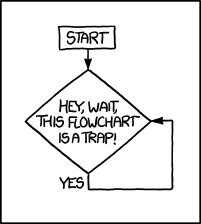
\includegraphics[scale=0.55]{trap}
        \end{figure}
    \end{columns}
\end{frame}

\begin{frame}
    \frametitle{Loops in C++}
    \subsection{Loops in C++} % (fold)
    \label{sub:loops_in_c}
    There are three types of loops in C++:
    \begin{itemize}
        \item the \texttt{for} loop,
        \item the \texttt{while} loop, and
        \item the \texttt{do} loop
    \end{itemize}
\end{frame}

\begin{frame}
    \frametitle{The \texttt{for} Loop}
    \section{The \texttt{for} loop} % (fold)
    \label{sec:the_texttt_for}
    \begin{columns}
        \column{0.5\textwidth}
        \begin{itemize}
            \item Easiest to understand because all its loop control elements are gathered in one place
            \item Executes a section of a code a fixed number of times
        \end{itemize}
        \column{0.5\textwidth}
        \begin{figure}
            \centering
            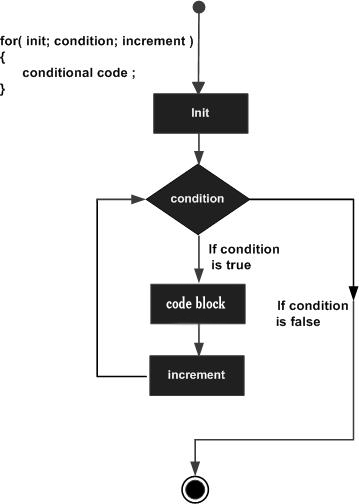
\includegraphics[scale=0.4]{for}
        \end{figure}
    \end{columns}
\end{frame}

\begin{frame}[fragile]
    \frametitle{The \texttt{for} Loop -- Syntax}
    \subsection{Syntax} % (fold)
    \label{sub:for_syntax}
    \begin{columns}
        \column{0.4\textwidth}
        \lstset{style=mystyle}
\begin{lstlisting}
for(init; test; update)
    {
       statement;
       statement;
       statement;
       statement;
    }
\end{lstlisting}
        \column{0.57\textwidth}
            \begin{itemize}
            \item Keyword \texttt{for} followed by parantheses that contain three expressions separated by semicolons
            \begin{enumerate}
                \item the initialization expression,
                \item the test expression, and
                \item the update expression
            \end{enumerate}
            \item These three expressions usually involve the same variable, also known as the loop variable
            \item The body of the loop, delimited by the left and right braces, is the code to be executed each time through the loop
            \end{itemize}
    \end{columns}
\end{frame}

\begin{frame} [fragile]
    \frametitle{The \texttt{for} Loop -- Solved Example 1}
    \subsection{Solved Examples} % (fold)
    \label{sub:for_solved_examples}
    \subsubsection{Solved Example 1} % (fold)
    \label{subsub:solved_example_1}
    \lstset{style=mystyle}
    \begin{lstlisting}
// demonstrates simple FOR loop
#include <iostream>
using namespace std;

int main ()
{
    int j;
    for(j = 0; j < 15; j++)
    {
        cout << j * j << endl;
    }
    return 0;
}
\end{lstlisting}
\end{frame}

\begin{frame} [fragile]
    \frametitle{The \texttt{for} Loop -- Solved Example 2}
    \subsubsection{Solved Example 2} % (fold)
    \label{ssub:solved_example_2}
    \lstset{style=mystyle}
    \begin{lstlisting}
// lists cubes from 1 to 10
#include <iostream>
#include <iomanip>
using namespace std;

int main()
{
    int num;

    for(num = 1; num <= 10; num++)
    {
        cout << setw(4) << num;
        int cube = num * num * num;
        cout << setw(6) << cube << endl;
    }
    return 0;
}
\end{lstlisting}
\end{frame}

\begin{frame}[fragile]
    \frametitle{Variation in \texttt{for} Loop}
    \subsection{Variation in \texttt{for} loop} % (fold)
    \label{sub:for_variation}
    \begin{itemize}
        \item Initialization can also be performed before loop expression
        \lstset{style=mystyle}
\begin{lstlisting}
int i = 1;
for(; i <= 5; i++)
\end{lstlisting}
        \item Update expression can also be placed within a loop body
        \lstset{style=mystyle}
\begin{lstlisting}
int i = 1;
for(; i <= 5;)
{
    cout << "i = " << i << endl;
    i++;
}
\end{lstlisting}
        \item If test expression is omitted, then the loop will run forever
        \lstset{style=mystyle}
\begin{lstlisting}
int i = 1;
for(;; i++)
{
    cout << i << endl;
}
\end{lstlisting}
    \end{itemize}

\end{frame}

\begin{frame} [fragile]
    \frametitle{The \texttt{break} Statement}
    \subsection{The \texttt{break} Statement} % (fold)
    \label{sub:the_break}
    \begin{itemize}
        \item Immediate exit from the loop
        \item Program continues with first statement after the loop block
        \item Used to escape early from a loop
    \end{itemize}
    \lstset{style=mystyle}
\begin{lstlisting}
for (x = 1; x <= 10; x++)
    {
        if (x == 5)
            break;
        cout << x << endl;
    }
    cout << "\n Out when x became " << x;
\end{lstlisting}
\end{frame}

\begin{frame} [fragile]
    \frametitle{The \texttt{continue} Statement}
    \subsection{The \texttt{continue} Statement} % (fold)
    \label{sub:the_continue}
    \begin{itemize}
        \item Skips remainder of the loop body
        \item Proceeds with the next iteration of loop
    \end{itemize}
    \lstset{style=mystyle}
\begin{lstlisting}
for (x = 1; x <= 10; x++)
    {
        if (x == 5)
            continue;
        cout << x << " ";
      }
    cout << "\n Skipped value 5" <<endl;
\end{lstlisting}
\end{frame}

\begin{frame}
    \frametitle{Exercises}
    \section{Exercises} % (fold)
    \label{sec:exercises}
    \begin{itemize}
        \item Write a program using \texttt{for} loop which displays the following shape \\ [0.2 in]
        * * * * * * * \\
        * * * * * * \\
        * * * * * \\
        * * * * \\
        * * * \\
        * * \\
        * \\
        \item Write a program using \texttt{for} loop which displays all the even numbers from a minimum number entered by the user to a maximum number entered by the user
    \end{itemize}
\end{frame}
\end{document}